\chapter{MULTIPLE OBJECT TRACKING}

\renewcommand{\headrulewidth}{0.5pt}
\renewcommand{\footrulewidth}{0.5pt}
\thispagestyle{plain}
\pagestyle{fancy}
\fancyhf{}
\fancyhead[L]{\textbf{CHAPTER 3}}
\fancyhead[R]{\textbf{Intelligent Traffic System}}
\raggedright
\fancyfoot[L]{From: ITM Vision}
\fancyfoot[R]{Page \thepage}

\section{Overview}
    Multiple object tracking can be viewed as a multi-variable estimation problem. Given an image sequence, we employ
    $s_t^i$ to denote the state of the i-th object in the t-th frame, $\textbf{S}_t = (s_t^1, s_t^2, ..., s_t^{M_t})$
    to denote states of all the $M_t$ objects in the t-th frame. Let \textbf{$s_{i_s:i_c}^i = \{s_{i_s}^i,...,s_{i_e}^i\}$} 
    be the sequential states of the i-th object, where $i_s$ and $i_e$ are respectively the first and last frame in 
    which target \emph{i} exist, and \textbf{$S_{1:t} = \{S_1,S_2,...,S_t\}$} to denote all the sequential states of all the 
    objects from the first frame to the t-th frame. Note that the object number may vary from frame to frame. \\ 
    \vspace{3mm}
    Correspondingly, following the most commonly used tracking by detection, or Detection Based Tracking (DBT) paradigm,
    we utilize $o_t^i$ to denote the collected observations for the i-th object in the t-th frame. $\textbf{O}_t=(\textbf{o}_t^1,\textbf{o}_t^2,...,\textbf{o}_t^{M_t})$ 
    to denote the collected observations for all the $M_t$ objects in the t-th frame, and $\textbf{O}_{1:t}=\{\textbf{O}_1,\textbf{O}_2,...,\textbf{O}_t\}$ 
    to denote all collected sequential observations of all the objects from the first frame to the t-th frame.
    \vspace{3mm}
    The objective of multiple object tracking is to find the “optimal” sequential states of all the objects, which can be 
    generally modeled by performing MAP (maximal a posteriori) estimation from the conditional distribution of the 
    sequential states given all the observations: 
    \begin{align}
        \hat{S}_{1:t}=\underset{S_{1:t}}{argmax}P(\textbf{S}_{1:t}|\textbf{O}_{1:t})
    \end{align} 
    Different MOT algorithms from previous works can now be thought as designing different approaches to solving 
    the above MAP problem, either from a probabilistic inference perspective or a deterministic optimization perspective. 

\section{Categorization}
    Categorization of MOT bases on: initialization method, processing mode and type of output.
    \begin{itemize}
        \item Initialization method: MOT devides into detection based tracking and detection free tracking
            \begin{itemize}
                \item Detection based tracking: Given a sequence, type specific object detection or motion detection (based on background modeling) is applied in each frame 
                to obtain object hypotheses, then (sequential or batch) tracking is conducted to link detection hypotheses into trajectories. Detection based tracking focuses 
                on specific objects and its performance relies heavily on accuracy of object detectors. Detection based tracking is more popular as it can deal with new 
                discovered and disappear objects automatically.
                \item Detection free tracking requires requires manual initialization of objects in each frame.
                    \begin{figure}[H]
                        \centering
                        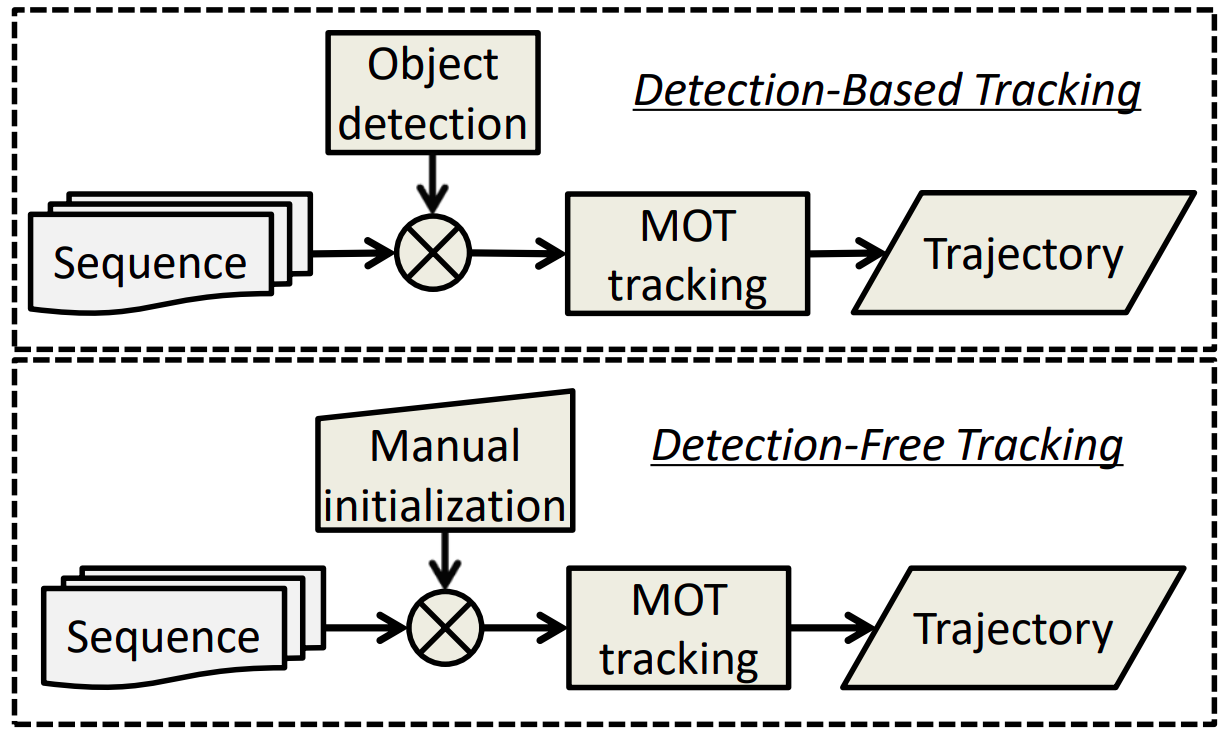
\includegraphics[width=0.6\linewidth]{img/MOT.png}
                        \caption{Pipeline of detection based tracking and detection free tracking}
                    \end{figure}
            \end{itemize}
        \item Processing mode: based on processing mode, MOT can be divided into online tracking and offline tracking problem. 
            \begin{itemize}
                \item An online model receives video input on a frame-by-frame basis, and has to give an output for each frame. This means that, in addition to the current frame, 
                only information from past frames can be used. Online tracking takes up-to-time observation and updates trajectories on the fly there for it is suitable for real time application.
                \item Offline models, on the other hand, have access to the entire video, which means that information from both past and future frames can be used. The task can then be viewed as an 
                optimization problem, where the goal is to find a set of paths that minimize some global loss  function. Offline tracking takes a batch of frames to process therefore it products delay results. 
                Since offline trackers have access to more information, one can expect better performance from these models. 
            \end{itemize}
    \end{itemize}
    Detection free tracking process data sequentially while in Detection based tracking, tracklet or detection response are often associated in batch. \\ 
    \vspace{3mm}
    Recently with the rise of deep learning, MOT can also devided into non-deep learning based methods and deep learning based methods. \\ 
    \vspace{3mm}
    In deep learning based methods, first CNN-based object detectors are applied such as Faster R-CNN and YOLOv3 to localize all objects of interest in input images. Then in a separate step,they crop the images 
    according to the boxes and feed them to an identity embedding network to extract re-ID features which are used to link the boxes over time. The linking step usually follows a standard practice which first 
    computes a cost matrix according to the re-ID features and Intersection over Unions (IoU) of the bounding boxes and then uses the Kalman Filter and Hungarian algorithm to accomplish the linking task. 
    MOT methods based on deep learning can be further devided into two-stage method and one-stage method. \\ 
    \vspace{3mm}
    The main advantage of the two-step methods is that they can develop the most suitable model for each task separately without making compromise. In addition, they can crop the image patches according to the 
    detected bounding boxes and resize them to the same size before estimating re-ID features. This helps to handle the scale variations of objects.The main drawback due to the fact that they are usually very 
    slow because the two tasks need to be done separately without sharing. \\ 
    \vspace{3mm}
    For one stage method, the core idea is to simultaneously accomplish object detection and identity embedding (re-ID features) in a single network in order to reduce inference time. However, the accuracy of the 
    one-shot trackers is usually lower than that of the two-step ones.

\section{MOT Components Overview}
    \subsection{Appearance Model}
        Appearance model includes visual representation and statistical measuring. Appearance model is important cue for affinity computation in MO. Visual representation: local features, region features, 
        Probabilistic Occupancy Map (POM), depth features, Statistical measuring: single cue \& multiple cues (five kinds of fusion strategies: Boosting, Concatenating, Summation, Product, and Cascading).
    \subsection{Motion Model}
        Motion model includes linear \& non-linear model. It aims to estimates the potential position of objects in the future frames, thereby reducing the search space.
    \subsection{Interaction Model} 
        Interaction model, also known as mutual motion model, captures the influence of an object on other objects. In the crowd scenery, an object would experience some “force” from other agents and objects. 
        Interaction model includes social force model \& crowd motion pattern model.
    \subsection{Exclusion Model}
        Exclusion model includes detection-level exclusion \& trajectory-level exclusion. Exclusion is a constraint employed to avoid physical collisions when seeking a solution to the MOT problem. It arises from 
        the fact that two distinct objects cannot occupy the same physical space in the real world.
    \subsection{Occlusion Handling}
        Occlusion is perhaps the most critical challenge in MOT. It is a primary cause for ID switches or fragmentation of trajectories. In order to handle occlusion, various kinds of strategies have been proposed such as: 
        part-to-whole, hypothesize-and-test, buffer-and-recover.
    

\section{Detection Based Tracking and End to End Tracking}

\section{SORT}

\section{Deep SORT}

    \subsection{Feature Extraction and Embedding}

    \subsection{Affinity Computation and Data Association}

\section{Metrics and Evaluations}

    \subsection{Conventional Metrics}

    \subsection{Update Metrics}